\documentclass{XDUthesis} %[draft]

\title{基于树莓派的显微成像系统}
\author{彭峰}
\date{2016年04月12日}
%题目拆分:用于封面
\septitleA{基于树莓派的显微成像}%如果论文题目长度<=11中文字符只需填此项即可B项空着
\septitleB{系统}%如果论文题目长度>11中文字符, 建议拆分为10+x or 11+x 将剩余x个字符填在此处。
\class{05121201}%班级号
\schoolnumber{05121214}%学号
\major{电子科学与技术}%专业
\school{物理与光电工程学院}%学院
\supervisor{刘杰涛}%指导老师

\begin{document}

% 摘要
% 中文摘要
\begin{abstract}
	
	{\large 没有放图上去,没有特意排版文字段落,仅看基本框架使用。没有引用等,后续更改,多数文字copy,简单充实下。}
显微成像的应用开始在越来越多的领域中得到应用。光学薄膜的表面粗糙度对其光学特性的测量精度有较大影响。在常见的加工生产过程中,薄膜表面的毛刺、划痕等都可能对精密产品的性能造成影响。为提高产品的光学特性的精度,对相应产品出厂前表面进行实时的、高精度的缺损情况测试具有实际重要意义。使用电子仪器的手段相比于传统人力目测检验方法,具有单位效率高、判定率高、可靠性高等特点,便于元器件表面缺损测试方面向现代微型组件化智能化发展。
本文依托ARM处理器平台设计了数字化显微成像技术处理系统,并对零部件表面的缺损情况进行了实时测试。此检测系统具有智能化、小型化、图像采集方便实时的特点,可以进一步提高产品出厂前合格率、降低后续产品返修率。整体上,采用索尼的堆栈式CMOS图像传感器IMX135,作为核心数字显微图像采集芯片,借助CSI-2接口将图像传至ARM主板,并利用ARM处理器完成显微图像的图像增强、图像识别等算法处理,并实现了显微图像的后续存储、归档和显示。存储、归档上可以放在存储卡或云端,通过HDMI或网络将图像传输到LED平板显示器上进行显示,达到实现系统集成化、桌面一体化、处理器实时处理的常见功能,同时备选两套方案,即可使用HDMI线缆将显微图像传输到桌面显示,利用以太网或802.11协议,借助路由也可以在异地通过互联网的方式,通过浏览器访问显示显微图像。更好实现产品缺损检测效果的远程实时控制功能。
本论文完成下面工作:
\begin{enumerate}
	\item 完成嵌入式显微成像系统的整体设计,包括光学显微成像子系统、图像显示处理子系统、上位机图像显示子系统等。
	\item 依据情况,设计显微图像采集的硬件设计方案、软件显示方案。分析技术要求、选型相应硬件,借助树莓派为主的ARM处理器平台,利用发布的CSI接口适配图像处理驱动和Web显示B/S方案,实时采集的图像通过CSI-2接口传输到基于ARM的主板,经过图像增强和图像滤波算法处理后,将相应图像显示出来。
	\item 对设计的ARM平台下的嵌入式显微成像系统进行相应的实验测试,在不同的光照强度下,对缺损的光学薄膜表面情况进行成像检验,改进系统不足,最后满足系统的整体设计要求。
\end{enumerate}


\end{abstract}
\keywords{数字显微成像, 光学薄膜, ARM  }

% 英文摘要
\begin{enabstract}
	Optical thin film and its products have been widely used in various fields. The surface roughness of optical thin film has a very important influence on the optical properties such as refractive index, surface scattering and so on. In the process of production and processing, the surface of fine scratches, stains, burrs and other will affect the performance of the products, therefore the process on the surface of the parts of real-time and accurate defect detection has important significance. The traditional manual visual inspection method has the disadvantages of large labor intensity, low accuracy, low efficiency, poor reliability, and so on. It can’t adapt to the needs of the development of modern production totheminiaturizationofintelligent. In view of the on-line detection of the surface defects of the optical thin film, the on-line detection system based on ARM processor is designed. The system has the characteristics of on-line, real-time and non-contact, which is very important for ensuring the quality and improving the production efficiency of the optical thin film products. CMOS image sensor IMX135 is used as digital microscope image acquisition part.Through the CSI-2 interface, the image is transferred to theARM processor. The images are processed and stored in the ARM processor. The image is processed and stored, and the image is transferred to the LCDscreenbyHDMIinterface.Thisthesismainlycompletesthefollowingwork
  

\end{enabstract}
\enkeywords{ARM, more, environments, skills}

% 往PDF属性里面写下关键词信息
\makeatletter
\XDU@setpdf@keywords
\makeatother

\maketitle

% 文章主要部分
{\tiny {\tiny }}\chapter{引言}
\section{选题背景及意义}
\subsection{选题研究内容(待改进)}
伴随着技术的革新和工艺上的不断进步,工业产品的表面精度检测要求不断提升,目前的缺陷检测方面技术开始越加复杂,各种的技术的工作方式和原理开始出现变更,体现在生活中的各个领域,高效的技术手段和实现方法直接决定了检测系统的可靠性和检测方法的便捷性。表面缺损一般是采用的加工方法和机器磨合有关联造成的,缺损的表象可能包括裂纹、气泡、、毛刺等缺陷。目前,光学显微镜仍然是使用最广泛的显微镜。但是在同时,传统人工方式仍然存在不少的局限性,如:使用人员使用显微镜时,视野不畅,容易造成视觉疲劳;在观察时,无法多人观察进行交流;不能对图像进行必要的处理,加强所需目标的对比度,快速存储、归档、显示。

数字图像处理技术和图像处理算法的不断发展,能够结合传统光学仪器和计算机技术各自的优势,更好的实现多种数据采样和处理功能,实现系统平台的图像处理,包括去噪,模块识别等功能。实现对显微镜中的显微图像实时/远程的监测,可以在公网上进行相应图片的显示。同时,关于数据的归档,显示和报表可进行额外的分析和处理、综合。在显微成像的数字化平台上,国内外一些仪器厂已经开始尝试研制,部分已有商品化的产品出售。相比和计算机直接进行显微镜连接的情况,使用本文的平台可以更方便的在小空间内使用,具有系统集成化和小型化的特性。\cite{machine}\cite{light3D}\cite{eletnature}


%本文主要说明了新型技术的使用和传统方式的对比。传统人工方式效率低,出错率较高,借助现有的图像增强和识别技术,可以加快验证进程,进一步匹配流水线。此外,阐述了实时检测的产品识别的价值和意义。
%关注光学成像部分,设计光学系统,实现图像的处理,归档,显示,性能报表等相关功能。借助,完成系统的图像处理部分,可包括去噪,模块识别等功能。此外,关于数据的归档,显示和报表可进行额外的分析和处理、综合。硬件选用上,考虑ARM系列市场份额持续上升,学习成本较低,适应于通用型应用,选用基于ARM的嵌入式处理器技术,其相比于FPGA和DSP,有通用性强,占用体积小,能耗低,性价比高,平台兼容性好等多方面特性。CPU为RISC架构,单一指令周期,长流水线,TDP可以做到较低,于是此处通用选型选用ARM作为主控。在成像方面的传感器上,选用手机上常见的摄像头模块,易于获得,接口选用高速串行的CSI接口,频率高,单位数据传输量大,在后续处理中完成图像的预处理,辨识问题图片的编号,同时放在云上备份,做到图片的后续存储归档。
%图像系统采集的硬件设计和选型。在硬件设计上,需要考虑成本分配,易用性,可扩展性,兼容性,平台性能,产品参数等多方面因素。此次主要需要借助GPU的图像处理,因此不考虑DSP和FPGA模拟处理和外接芯片的方式,在版型上,为了库移植的方便以及资料的充分情况,决定选用raspberrypi老版本。
\subsection{解决问题(是否缩减到前面一小节)}
硬件成本的不断下降使曾经昂贵的技术使用更加广泛,显微成像的单一器具已经开始应用在生活的部分方面,在此基础的改进上,增加数据的处理模块,在不同指标不同场合的跟进测试,是目前的一个研究热点。

在此需求上,本文设计了基于树莓派的数字显微成像系统,尝试在缺陷材料上进行进一步测试。在设计中,选用了索尼的第二代BSI光照CMOS图像传感器IMX135,利用低压差分信号抗干扰来提高信噪比,使图像成像效果更佳。


\section{国内外研究现状}
\subsection{显微成像国内外发展现状}
显微镜的起源较早,但是在后期才发展快速。早在2500年前的《墨经》中,就已经有了凹透镜的记载,然而凸透镜的发展却一直没有进展。直到16世纪末期,荷兰的眼镜商詹森( Zaccharias Janssen) 和他的儿子尝试了一次将两个凸透镜放入到同一个镜筒中,发明了人类历史上第一个光学显微镜。而后在1609年,著名的天文学之父伽利略在这个实验的基础上,分解出相关的物理学原理,并依据自身的理论发明了更好聚焦的显微镜。

而后的列文虎克将放大倍数大大的提升了一截,第一次能够发现微观的生物和非生物现象,出版了极多的论文,同时极大的推进了生物学的发展。后之显微镜之父,罗伯特﹒虎克仿制了一台与列文虎克一样的显微镜,证实了水中微小微生物的发现,1830年,利斯忒 (Joseph Jackson Lister,1786-1869) 用几个有特定间距的透镜组减小了球面像差,从而进一步改进了显微镜。而后,1872年德国的数学家和物理学家 Ernst Abbe 改进了玻璃的制造和生产工艺,改进并生产出有均一折射率的光学级玻璃。\cite{microimaging}\cite{microimagingelc}

受到衍射限制,光学显微镜的分辨率达到显微镜的分辨率极限,即:
\begin{center}
	$ R = \lambda/(n \cdot \sin(\alpha)) $ 
\end{center}
这里的 R 是分辨率,$\alpha$ 是孔径张角,$\lambda$ 是波长 , $n\cdot\sin(\alpha)$ 是数值孔径,$n$是折射率。 
	

\subsection{光学薄膜检测的发展现状}
 光学薄膜广泛应用于液晶显示屏、触摸屏、太阳能电池板等行业,对表面质量有极高的要求,如何保证其质量要求,必须要借助有效的的检测手段进行检测。与其他如金属、印刷品、玻璃制品等行业同类检测技术相比,由于薄膜的高透光性、缺陷尺寸极小、薄膜运行速度高,致使曝光时间短,CCD感光不足,图像整体偏暗,最终导致目标与背景的灰度级差极小。\cite{CCDCMOSf}传统的人工目视检验或离线抽检方法劳动强度大、精度低、效率不高、可靠性差等缺点,无法适应现代化的生产要求。


起源

商业应用

检测

完善

重要性

\section{本文主要任务和安排}
\subsection{主要任务和安排}
硬件成本的不断下降使曾经昂贵的技术使用更加广泛,显微成像的单一器具已经开始应用在生活的部分方面,在此基础的改进上,增加数据的处理模块,在不同指标不同场合的跟进测试,是目前的一个研究热点。

在此需求上,本文设计了基于树莓派的数字显微成像系统,尝试在缺陷材料上进行进一步测试。在设计中,选用了索尼的第二代BSI光照CMOS图像传感器IMX135,IMX135 有最高60fps,4208x3120的分辨率,小至1umx1um的像元尺寸,总像素为1300万,利用低压差分信号抗干扰来提高信噪比,使图像成像效果更佳。
在研究过程中,更希望是显微成像方面在传统设备转向电子化,数字化,智能化,互联网化的一种可行性的尝试。进一步改善整体流程,加强后续的研究和信息处理的长尾方式,提高部署的高效性,降低生产成本。

	
\subsubsection{具体章节结构}
%讲实际的情况了解。
本文主要的内容设置如下:

第一章对本文的研究原理和背景做基本的阐述,希望解决的问题。并查阅相关显微成像和光学薄膜的国内外发展现状,在此基础上进一步改进,介绍本文的主要结构和目前安排。

第二章设计显微成像系统硬件部分,对显微成像的光学原理做出阐述,并进行目镜物镜的选型。图像传感器功能和类型性能比较选型,数据传输接口的比较,显示处理方式的比较和选择,设计出一个较完整的低耦合化方案。

第三章对显微图像处理平台进行系统设计,查阅研究了相关CSI的接口在树莓派的驱动程序,介绍V4L2框架的应用和使用。并分析图像算法的在预处理和处理上的研究,包括线性滤波、中值滤波、高斯滤波,边缘检测等方法,并研究了显微图像的相关拼接算法,设计了阈值分割和像素投影算法。最后在Web上展示处理后的图像,同时可以查阅前期归档后的图像。

第四章设计显微成像的实验测试系统,验证系统可行性,并依据照明光线变量验证可以达到的系统精度,满足系统的测试要求指标。

第五章为论文的总结和展望,总结主要研究学习工作,提出了可能存在的问题和未来的改进思路方向。


\subsection{本章小结}
本章首先介绍了选题的来由和解决的问题,简要说明了显微镜的发展史,介绍了显微成像的光学结构和组成原理,同时简单说明了光学薄膜检测的问题和传统方式。在介绍基本情况之后,详细说明论文的架构安排、学习的内容和完成的主要工作。

\chapter{显微成像系统整体方案设计}
本显微成像检测系统由光学模块、图像处理模块、图像采集模块、图像归档显示模块等构成。在整体设计流程中,关键的技术包括图像传感器的分析与选择、图像主处理器及预处理器的选择等。本章在光学基础上,根据需求和情境重点分析了各个不同模块需要的硬件优势方面和选型,并对此进行较为详细的讲述。可见的一个分类的图\ref{fig:module_1}示如:
\begin{figure}[h]
\centering
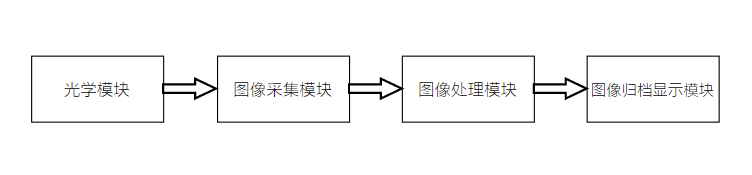
\includegraphics[width=0.7\linewidth]{Figure/module_1}
\caption{模块介绍}
\label{fig:module_1}
\end{figure}


\section{显微基本原理}
\subsection{光学成像原理}

显微镜的成像如图\ref{fig:micro_1}所示,小物体AB在物镜的焦距之外,人眼在另一边的距离除观察,AB形成放大倒立的实像A'B',而这一实像正好在目镜的焦距以内的附近处,再一次经过目镜放大之后,在明视距离d处形成正立虚像A"B"\cite{lightxidian}。


\begin{figure}[h]
	\centering
	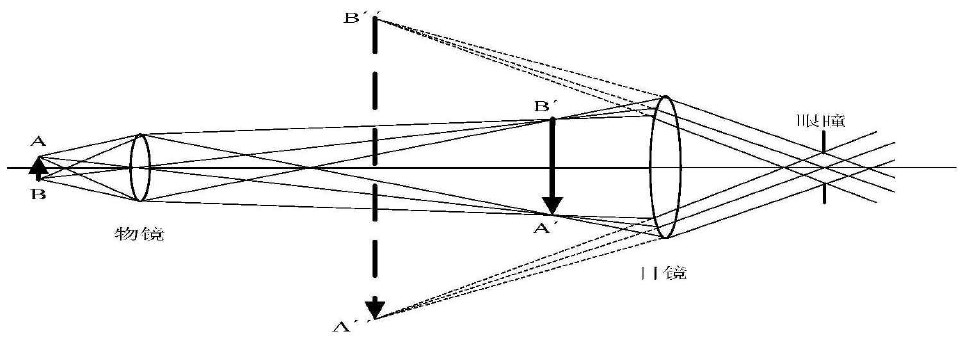
\includegraphics[width=0.7\linewidth]{Figure/micro_1}
	\caption[显微镜成像光路图]{显微镜成像光路图}
	%\caption{显微镜成像光路图}
	\label{fig:micro_1}
\end{figure}

显微镜的视觉放大率定义为:

\begin{equation}
\label{j2}
J = l_{0}\cdot d / f_{1}f_{2}
\end{equation}

式\ref{j2}中 $d$ 是明视距离,$l_{0}$为物镜到目镜的距离, $f_{1}$ 为物镜的焦距, $f_{2}$ 为目镜的焦距。此处的角放大率为物镜的线放大率和目镜的角放大率的乘积。
数值孔径的孔径角的正弦与透镜和物体之间介质的折射率的乘积,而显微镜的分辨率与光的波长和物镜的数值孔径有关,波长越短,数值孔径越大,分辨率越大\cite{fenbianlv}。


\subsection{显微镜结构构造}
普通光学显微镜的构造可分为两部分:一为机械装置,一为光学系统 。机械装置由镜座、镜筒、物镜转换器、载物台、推动器、粗动螺旋和微动螺旋等部件组成。光学系统由目镜、物镜、聚光器、光源、滤光片、虹彩光圈等组成。
一个典型显微镜如图\ref{fig:mi_1}所示。
\begin{figure}[h]
\centering
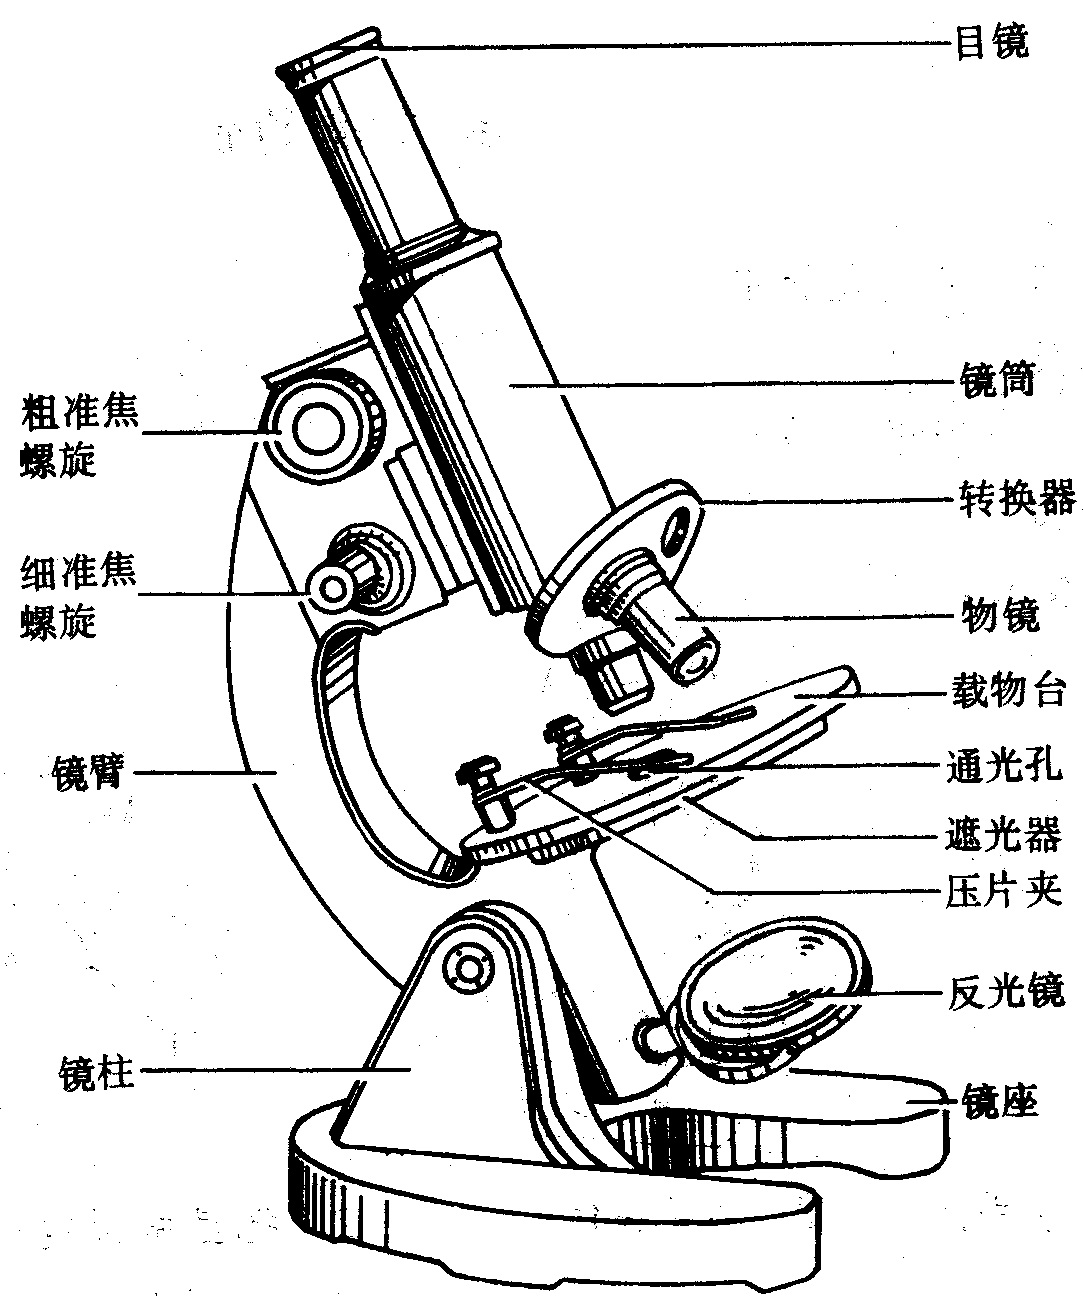
\includegraphics[width=0.7\linewidth]{Figure/mi_1}
\caption{典型显微镜结构图}
\label{fig:mi_1}
\end{figure}


物镜是决定显微镜性能的最重要部件,安装在物镜转换器上,接近被观察的物体,故叫做物镜或接物镜。通常目镜由上下两组透镜组成,上面的透镜叫做接目透镜,下面的透镜叫做会聚透镜或场镜。聚光器也叫集光器。位于标本下方的聚光器支架上。它主要由聚光镜和可变光阑组成。其中,聚光镜可分为明视场聚光镜和暗视场聚光镜。反光镜是一个可以随意转动的双面镜,直径为50mm,一面为平面,一面为凹面,其作用是将从任何方向射来的光线经通光孔反射。平面镜上反射光线的能力较弱,适合在光线较强时使用,凹面镜反射光线的能力较强,适合在光线较弱时使用。

\section{显微成像处理平台器件选型}
\subsection{显微镜头物镜选型}
常见的物镜通过像差校正程度的不同,可划分为:消色差物镜、复消色差物镜,半复消色差物镜和特种物镜。这里选用最简单的消色差物镜,通过减少透镜的片数降低选择的难度。

下面对物镜中常见的一些重要的参数和公式做出解释。

物镜的数值孔径:
\begin{equation}
\label{NA}
\mathit{NA} = n\sin \alpha 
\end{equation}

式\ref{NA}中,$\alpha$代表物镜在物方的孔径半角,$n$ 表示物空间的介质折射率。增加数值孔径的方式可以通过增加透镜的孔径或者采用焦距较短的物镜来增大孔径半角$\alpha$。

两物镜的最小分辨距离表现为:
\begin{equation}
\label{one}
\mathit{K}\lambda / n\sin \alpha 
\end{equation}

在式\ref{one}中, $\lambda$为成像光线的波长,$n$为测试物周围物质的折射率, $\mathit{K}$为数值, 由式\ref{NA}可知,$n\sin \alpha$即$\mathit{NA}$常表示为物镜的数值孔径。数值孔径越大,能够分辨两物点的最短距离则越小,分辨率越高。

\begin{equation}
\label{dd}
d/f \approx  1.22/D
\end{equation}
\begin{equation}
\label{nd}
ndsin \alpha=n'd'sin \alpha'
\end{equation}


式\ref{dd}中,,考虑到实际因素,考虑式\ref{nd}条件,其中$n$为物空间折射率,$n'$为像空间折射率,在空气介质中,取 $\alpha'$为 1;$\alpha$ 是光线在物空间的孔径角,$\alpha'$是对应的像空间共轭点的孔径角;$d$ 为物平面上两点的 间距,$d'$为像面上两像点中心间距,$f$ 为透镜的焦距。考虑到斜入射光线的影响,修正 后的公式表示为:$d=0.5/NA$,其中 $nsin\alpha$ 即物镜的数值孔径。 

通过减小对饮照明光的波长和增大数值孔径的方式可以提高物镜的分辨能力,通常试验中使用波长较短的黄绿光提升分辨能力。

在物镜的放大倍率上,通常为人眼明视距离处的分辨出0.15到0.30mm大小,一般认为是0.20mm。如果过小的话,将不能良好分辨。

最后的设计为物镜的放大倍数为10,光源的照明波长认定为550nm,透镜数值孔径由式\ref{NA}测得为0.6。最后判定物镜的焦距大致范围,便于物镜选型和后期的进一步微调。

\subsection{图像传感器的选型}
固体图像传感器已经广泛地应用于生活各处,包括像电子照相机、DV、智能监控、手机、平板和摄像头等。固体图像传感器是利用半导体材料的内光电效应原理制成的光电转换器件,依据工艺结构可以分为两大类:一类是电荷耦合器件(CCD)图像传感器;另一类是互补金属氧化物(CMOS)图像传感器。两种目前常见的图像传感器都是上世纪60年代开始研制,在当时由于CCD图像传感器灵敏度更高、噪声较低而成为当时图像传感器的主流。而CMOS图像传感器由于工艺上的提升限制,长时间未能摆脱光照灵敏度低、噪声无法下降和图像分辨率低等不足。于此同时,CCD图像传感器由于敏感元件和信号处理电路无法集成在同一芯片上,使得照相机体积大、功耗大\cite{CCDCMOSf}。
进入新世纪,时间发展,随着互联网向移动互联网的转移,智能手机的发展十分迅速,由于CMOS图像传感器却有集成度高、体积小、功耗小和造价低等优点,十分适合在手机上进行集成,考虑到两种图像传感器的技术特点和缺点改进方式,随集成电路设计技术和迭代工艺水平的提高,CMOS图像传感器过去存在的缺点,现在开始逐渐进行技术攻关,常见的背照式结构让CMOS图像传感器在光线摄入上有长足的发展,而且它其固有的特点更是CCD器件所无法比拟的,因而它再次成为研究和工业需求的热点。
\subsubsection{CMOS和CCD的比较}
CCD和CMOS两者在多个维度上有着较大特性上的差异:

1.系统集成 \\

CMOS图像传感器易于在SoC上集成,便于在同一芯片中同时进行内部的信号降噪、数据整合和数据处理,片上数据传输率高,与周边电路的整合性高,更可可将与信号处理器整合在一起,如图所示,便于大幅度减小对应模块的主板面积占用。考虑到 CCD 和 CMOS 两者采用不同的制造工艺,所以 CCD 难以装入SoC。因此,一般认为CMOS图像传感器可以广泛使用在各个嵌入式领域。

2.性能特性\\

在实际应用方面,性能特性是进行芯片选型取舍的极为重要的因素。CMOS图像传感器由于多个放大器的存在,不同一组生产的放大器放大情况有细微差异,导致最终的图像输出噪声较多。此外,由于集成度高的缘故,各元件、电路之间距离较近,相互之间的光、电、磁干扰显得严重,噪声对图像质量影响很大。在需要的电源数方面,相对于CCD图像传感器需要三或四组电源,CMOS图像传感器则只需一个即可。
而且CMOS图像传感器利用3.3V电源即可驱动,相比之下电源消耗量比CCD图像传感器低。因此,在功耗和电压方面,CMOS图像传感器比CCD图像传感器在小型化嵌入式设备中有更大的优势。此外,CMOS信号读取的方式较为简易,电路设计相应也可简单。

3.可靠性\\

两种图像传感器在商用及工业应用领域具有等价的可靠性。在极端恶劣的应用环境中,由于CMOS图像传感器充分提高系统集成度、降低模块间耦合,借助设计良好的封装和焊接技术,其可靠性优于CCD图像传感器。

%\caption{CCD和CMOS特性比较}\label{Tab:cmos1}
\begin{table}[htbp]
	\caption{\label{tab:cmosccd}CMOS和CCD对比}
	\centering
%	\label{table:cmosccd}	
 \begin{tabular}{|L{2.2cm}|C{4cm}|R{4cm}|}
%\toprule[1pt]
\hline
	& CMOS图像传感器 & CCD图像传感器 \\ \hline
	\rowcolor{mygray} \hline
	感光灵敏度 & 低 & 高 \\ \hline
	噪声电子数 & 200 & 50 \\ \hline
	\rowcolor{mygray}
	电路集成度 & 高 & 低 \\ \hline
	工艺难度 & 小 & 大 \\ \hline
	\rowcolor{mygray}
	成本 & 低 & 高 \\ \hline
	功耗 & 低 & 高 \\  \hline
	\rowcolor{mygray}
	ADC  & 片内集成  &  片外设置 \\ \hline
 \end{tabular} 
\end{table}

\subsubsection{图像传感器的选择}
在图像传感器的选择上,需要考虑成像质量,分辨率,集成度,接口匹配,适配度等几项重要指标。由上面的比较可以知道,CMOS图像传感器的集成度远
远优于CCD图像传感器。CMOS图像传感器可将多个处理器,控制器模块集成到一块芯片上,直接输出数字信号,减小开发难度。而在成向质量,分辨率上,两者均能达到要求,最关注的集成性,低功耗,采样速度高等特点,CMOS图像传感器占有很大的优势。

在考虑到成本问题之后,决定选用CMOS传感器作为图像采集的模块。
这里经过多次比对,决定选择SONY的IMX系列传感器。SONY最近数年在CMOS技术上的大幅度改进使得CMOS传感器的图片质量开始接近数码相机的质量。尤其是背照式技术和堆栈式技术的使用,让CMOS图像传感器进一步接近CCD图像传感器的功能。最后考虑选用IMX135进行相关实验。


\subsection{图像处理方案研究}
实时图像处理系统要求系统需要在有限的时间内完成大量数据的运算。可尝试实现的实现有下面几种:基于PC的数据处理,基于DSP的数字信号处理,基于ARM的通用事务处理。

(1)在PC上的数据处理:是常见的图像处理方式,利用高级编程语言进行算法编程,但在实时图像数据处理上可能需要占用CPU大量的浮点计算能力,然而CPU更适合进行整数计算,在PC中大量的浮点运算通常放在GPU中运行。

(2)基于DSP的数字信号处理:通用可编程的DSP在嵌入式领域中有数字信号处理精度高,速度快,一定的编程性等优势,相对而言算法较为复杂,在高速图像处理中一定优势。

(3)基于ARM的数据处理:随着VLSI技术的不断进步,ARM在近年来在嵌入式领域上的使用比率逐渐上升,市场上借助手机的快速发展ARM的出货量和迭代速度变更极快。此外,ARM有比较强的事物管理功能,可利用通用的语言和驱动,也可方便设计图形界面和应用程序。进一步的,随着硬件功能的不断加强,ARM系列中Cortex-M0处理器开始能以较高的性价比和单片机进行比较。


下面表\ref{table:tabarm}将三者的情况作出下面的对比。


%\begin{tabular}{>{\sf }llll}    %
\begin{table}[htbp]
	\centering
	\caption{ARM与其他处理器类型比较}
	\label{table:tabarm}
\begin{tabular}{l|l|l|l|l}
	\toprule
	\rowcolor{mygray}
	    & 主要实现方法   & 速度 &  性价比 & 应用优势 \\
	\midrule
	ARM     & 高级编程语言  & 较快 & 高  & 通用软件  \\
	\rowcolor{mygray}
	DSP       & 专用指令  & 快 & 中等 & 高精度计算 \\
	PC         & 高级编程语言  & 中等 & 低  & 通用软件 \\
%	\rowcolor{mygray}
%	Steel/Iron   & 450  & 25.0 & 234 \\
%	Lead         & 130  & 26.8 & 323 \\
%	\rowcolor{mygray}
%	Ice ($-$10) & 2100 & 38 & 323 \\
	\bottomrule
\end{tabular}
\end{table}

综合上述因素,探究到ARM有着良好的事物管理的功能,可以实现较多的PC端的功能,内容和课扩展性比较大。DSP主要用于高精度计算,如加密解密,调制解调等,有着极好的数据处理能力和较高的运行速度。PC端可以通过通用型计算的特点实现要求功能,但在实际使用中,GPU的调用功能不明显,CPU的浮点运算能力较低,如添加显卡则又一步增加了成本和功耗,且不利于实现小型化,功能化的特点。加之现在的趋势是单一的DSP功能正在被有较强信号处理功能的ARM取代,考虑使用ARM。

%区别是什么?:ARM具有比较强的事务管理功能,可以用来跑界面以及应用程序等,其优势主要体现在控制方面,而DSP主要是用来计算的,比如进行加密解密、调制解调等,优势是强大的数据处理能力和较高的运行速度。FPGA可以用VHDL或verilogHDL来编程,灵活性强,由于能够进行编程、除错、再编程和重复操作,因此可以充分地进行设计开发和验证。当电路有少量改动时,更能显示出FPGA的优势,其现场编程能力可以延长产品在市场上的寿命,而这种能力可以用来进行系统升级或除错。


\subsection{数据传输接口介绍}

\begin{figure}[h]
	\centering
	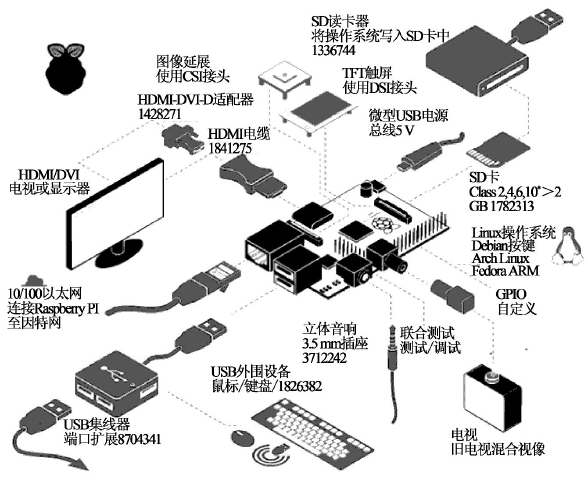
\includegraphics[width=0.7\linewidth]{Figure/rasp_3}
	\caption{树莓派基本硬件接口}
	\label{fig:rasp_1}
\end{figure}

如图\ref{fig:rasp_1}所示,树莓派包含的接口很多,包括USB电源接口、SD卡接口、GPIO、$I^{2}C$、USB2.0接口、CSI-2接口、HDMI接口、SVideo接口、以太网接口、3.5mm音频接口等。更可以通过USB接口连接分线器和鼠标键盘摄像头等实现扩展功能\cite{IoT}。

CSI属于MIPI标准之下。MIPI是一个比较新的标准,其规范也在不断修改和改进,目前比较成熟的接口应用有DSI(显示接口)和CSI(摄像头接口)。CSI/DSI分别是指其承载的是针对Camera或Display应用,都有复杂的协议结构。
CSI-2是一个单或双向差分串行界面,包含时钟和数据信号。CSI-2的层次结构:CSI-2由应用层、协议层、物理层组成。
由于串行接口一般采用差分结构,利用几百mV的差分信号,在收发端之间传送数据。串行比并行相比:更节省PCB板的布线面积,增强空间利用率;差分信号增强了自身的EMI抗干扰能力,同时减少了对其他信号的干扰;低的电压摆幅可以做到更高的速度,更小的功耗。

USB是连接电脑系统与外部设备的一种串口总线标准,也是一种输入输出接口的技术规范,被广泛地应用于个人电脑和移动设备等信息通讯产品,并扩展至摄影器材、数字电视(机顶盒)、游戏机等其它相关领域。目前含有多种型号。

以太网(Ethernet)是一种电脑局域网技术。IEEE组织的IEEE 802.3标准制定了以太网的技术标准,它规定了包括物理层的连线、电子信号和介质访问层协议的内容。以太网是目前应用最普遍的局域网技术,取代了其他局域网标准如令牌环、 FDDI 和 ARCNET 。这里用来连接互联网。

高清多媒体界面是(HDMI)一种全数字化影像和声音发送接口,可以发送未压缩的音频及视讯信号。HDMI可以同时发送音频和视讯信号,由于音频和视讯信号采用同一条线材,大大简化系统线路的安装难度。通过HDMI接口方便的连接到显示器进行图像显示。



\section{系统平台选择搭建}
%B/S(Browser/Server)架构,是浏览器和服务器的通信连接模式。在这一结构下,用户通过浏览器完成绝大多数的显示和回调,数据处理和归档还是主要通过服务器实现。这样可以大大简化的任务,减轻了系统维护与升级的成本,为用户的使用带来方便。但是,该方案有着系统运行速度和稳定性不够高的局限性。
%C/S(Client/Server)架构,即客户机和服务器的通信连接模式。它属于应用软件系统,充分利用客户端和服务器端的硬件环境,具体的运算和数据的处理被放在客户端,从而使客户端变得很“胖”,一般称为“胖客户机”;相对地,服务器端的任务较轻,称为“瘦服务器”,这样将任务合理分配到Client端和Server端来实现,降低了系统的通讯开销。
常见的架构方式包括B/S架构和C/S架构。B/S架构,是浏览器和服务器的通信连接模式。在这一结构下,用户通过浏览器完成绝大多数的显示和回调,数据处理和归档还是主要通过服务器实现。这样可以大大简化的任务,减轻了系统维护与升级的成本,为用户的使用带来方便。但是,考虑到网络的时延等,该方案有着系统运行速度和稳定性不够高的局限性。C/S架构,即客户机和服务器的通信连接模式。它属于应用软件系统,充分利用客户端和服务器端的硬件环境,较为常见的是将具体的运算和数据的处理被放在客户端,从而使客户端变得很“胖”,一般称为“胖客户机”;相对地,服务器端的任务较轻,称为“瘦服务器”,和操作系统的连接较为紧密\cite{bscs}。

相对于C/S模式,B/S模式显著的特点是浏览的跨平台操作,方便使用,考虑到跨平台的优势,所以目前越来越多的平台功能特性放在B/S架构下\cite{bshome}。
\chapter{显微图像处理平台系统设计}
本设计中采用了树莓派板 ARM 处理器,运用板中的 CSI-2 串行接口,将 IMX135 相机采集的显微图像传输至 BCM2836 处理器,在图像处理器 GPU 中进行数据的编 解码,对图像进行降噪、图像增强等处理,并以 H.264 格式的视频格式存储在 SD 卡 上,并通过 HDMI 接
口在显示器上播放显示,采用基于误差修正的算法对图像进行 缺损检测。树莓派板的硬件框图系统如图 4.1 所示。
\section{树莓派平台简介}
显微处理系统的主控核心采用开源的树莓派硬件系统,树莓派是一款基于开源的 Linux 操作系统的单板式计算机,其电路板尺寸只有一张银行卡大小,它起源于英国 的树莓派基金会,项目的发起者厄普顿其本想利用廉价硬件和自由软件激发在校学生 的计算机编程能力。第一版树莓派于 2012 年由英国剑桥大学正式向外界发布,现已 经发行至最新的第二代 B+型号

\section{图像传感器接口驱动程序}
\subsection{接口驱动简介}
V4L2 是 Linux 操作系统下摄像头驱动开发的协议,在深入分析了 V4L2API 中的 数据结构及 V4L2 驱动框架后,利用 V4L2 的框架进行了 CSI-2 摄像头的驱动设计。 
\subsection{V4L2驱动框架协议了解使用}
V4L2 中包含一整套的数据结构和驱动回调函数[39],下面对其进行了介绍。 (1)在 Linux 操作系统内核中,系统目录中的 linux/videodev2.h 函数封装库中 包括了开发过程中常用的数据结构体。如下列出常用的结构体并加以说明。


\section{显微图像预处理}
\subsection{预处理图像算法研究分析}

。。。均值,中值,高斯
设计双线性插值法、边缘
检测法和信号相关插值法三种格式图像转换算法,并分别对转换后的图像
质量进行了评估,最终确定采用信号相关插值法;研究了显微图像拼接算法,设
计了阈值分割与像素投影相结合的方法,实现了显微图像的无缝拼接

\section{实时图像处理算法分析}
融合算法
阈值分割算法

\section{上位机图像显示处理}



\chapter{显微成像系统的检测实验}

通过搭建实验检测平台,对光学薄膜的表面缺陷通过进行观测检测验证。对照本 显微成像检测系统的原理框图搭建实验平台,通过显微成像实验平台,实验完成对照 明光源的位置设置、显微图像采集格式的设置、树莓派接口通信的调试,以及对图像 数据采集传输与控制进行测试,验证了光学薄膜表面缺陷检测系统具备可行性。

\section{薄膜表面缺陷检测测试}

\subsection{实验仪器介绍和安装}
巴拉巴拉拔凉拔凉

安装

\subparagraph{硬件环境搭建}
首先组装实验装置平台,把设计的显微镜头和设计的 CMOS 驱动板通过 CS 口连 接起来,CMOS 驱动板的数据输出采用 FFC 软排线连接,组装好后的镜头如图 5.1 所示。
显微系统的照明光源采用环形白色 LED 的反射式照明,根据外界不同的环境光 照,可以调节照明 LED 灯的亮度,以适应不同透明度的薄膜的照明要求。采集不同 光照强度下的显微图像,选取具有最佳对比度的图像作为最终需要识别处理的图像。 
\subparagraph{软件系统设置}

搭建的实验系统平台如图 5.2 所示,连接显微镜头和 CMOS 采集板,采用反射式 的照明方式,打开上位机软件界面,并调节好显微镜焦距,观测镜片表面的薄膜,如 图 5.2 所示。
%\subparagraph{使用方式解释说明}

\subsection{缺陷检测结果分析}
在显微成像系统测试中,选取了实验室最常用的光学透镜的表面薄膜,观测了增 透膜和增反膜表面的缺陷程度,对表面出现的缺陷进行了分析。调整不同的光照方式, 对同一片增透膜进行了多次检测,以消除光照对检测误差的影响,采集到不同的薄膜 显微图像,并对传输上来的图片进行了图像预处理,采用均值滤波算法滤除高斯噪声, 并对图像进行二值化处理,对采集的多幅图像进行比较选择,排除对焦不同等差异条 件。采集到的薄膜表面的显微图像原始数据。
在上位机上对显微图像采用中值滤波进行图像降噪预处理,处理 结果如图 5.4 所示。
采用阈值分割处理算法对预处理过的图像做缺损检测处理,选定标准完整的薄膜 表面图像作为标准背景图,将显微系统采集到的带有缺损的薄膜表面图像与之对比, 对缺陷图像进行阈值分割处理,并截取放大显示识别出的典型的缺陷形状,选取记录 结果如下所示。

对薄膜的缺陷检测实验中,CMOS 相机采集的速度在 1080P 格式下达到每秒 30 帧,通过 CSI 接口传到显示器,实现了对薄膜的实时检测和识别,还能够通过网口传 到局域网实现远程缺陷检测。相比传统的缺陷检测系统,整个缺陷检测系统硬件上采 用了最新的 ARM 处理器,选用最新的 CMOS 图像传感器 IMX135,并通过 CSI-2 串 行接口输出图像,实现了高速实时的检测特点。整个检测系统结构紧凑,Raspbian 操 作系统可更新升级,实现了微型化智能化的检测特点。
\subsection{本章小节}
本章搭建了基于树莓派处理器的显微成像系统平台,选用不同光照强度的光源进 行照明,测试了实验室的光学薄膜表面的缺陷,验证了该系统的实时检测性能,并对 采集的薄膜表面的图像进行处理,识别出缺陷的类型和形状,达到了系统的总体设计要求。

\chapter{总结与展望}
\section{论文工作总结}
对光学薄膜的存在缺陷。。。。。。
\section{未来发展展望}
工工艺也有进一步提升的空间。 (3)在对图像处理进行算法分析方面,文中的图像的融合算法和基于误差修正 的分割方法虽然取得了预期效果,但是还存在进一步提升的空间,提升算法的智能化 处理和算法效率。 (4)在对显微图像的缺陷识别方面,对光学薄膜表面缺陷图像处理时缺陷提取 的有效性还需要进一步研究,需要针对图像缺陷的机制进行深入研究,对不同的缺陷 类型进行更好识别,以此提高该检测系统对光学薄膜缺陷图像的识别率。

% 致谢
\begin{thanksfor}
	
时光飞逝,转眼间本科阶段的学习和生活即将划上句号,4 年的本科学习虽然辛苦,
但能够学到知识却使我倍感快乐!在论文撰写完成之际,深深地感谢这段时间里给予我
关心和帮助的许多人。 

我首先要感谢我的导师刘杰涛讲师,在攻读学士学位期间,刘老师在某某等方面都给予我无私的教诲、悉心指导和无微不至的关心,他时时关注我的课题
研究进度,并敦促我及时完成我的毕业论文。刘老师治学态度严谨、学识渊博,这种严
谨的做学问的态度对我未来的学习、工作和生活都将产生深远的影响。 
感谢我的学长某某某,某某某,某某某等人陪我一起走过什么鬼阶
段,大家在一起上课学习交流的时光让我终生难忘。更要感谢他们在学术上给予我的帮
助和指导,使我能够顺利地完成论文。 

感谢实验室全体同窗们的热情帮助和支持,感谢刘晨、张琦、李海燕、李纯、韦迅、
任明溪、金辉、赵双全、孙美玲、殷梦妮、郭灵燕、刘明华、刘钦堂、孙志远、冯进玫、
隋毅、杨鹏、孙海、徐森、刘柏森等人共同营造的和谐、浓厚的学术氛围,和他们在一
起学习使我感到无比快乐,和他们的讨论使我受益匪浅。 
感谢我的其他同学和其他朋友,正是因为有了各位的扶持和陪伴,我的生活才能如此
的丰富、充实。 

感谢在座的各位领导和同事在此期间给予我充分的关心、帮助、理解和支持,对此表示由衷的感谢。
感谢物理与光电工程学院的很多老师在我学习期间和课题研究过程中给予我的热
心指导和无私帮助,谢谢你们! 

在我本科学习期间,要特别感谢我的家人尤其是我的父母给予我的无私帮助,正是他们对我的理解、支持和关心,才使我能够静下心来地学习、轻松地生活,良好的地
完成学业。 

寥寥数语难以充分表达我的感激之情,最后在这里祝大家万事顺意、身体安康。 

\end{thanksfor}

%参考文献
\phantomsection%生成该页的链接
\addcontentsline{toc}{chapter}{\bibname}
\bibliographystyle{XDUbib}%plain ieeetr
\bibliography{ThesisFiles/one}%在正文中必须引用,才能显示对应的参考文献

% 附录部分
\appendix
\chapter{网页索引}
%这里是附录的数据部分,作为测试;来看个公式编号对不对,如式\eqref{Eq:ApEq1}所示。

%\chapter{网页索引}
附录部分记录相关的知识网页,便于索引和查看。



https://www.raspberrypi.org/documentation/usage/camera/python/README.md 
   
https://www.raspberrypi.org/documentation/usage/camera/raspicam/raspistill.md

https://www.raspberrypi.org/forums/viewtopic.php?t=62364    

http://www.rs-online.com/designspark/electronics/blog/content-20

https://github.com/hypriot/rpi-kernel    

https://github.com/raspberrypi/tools  

https://www.djangoproject.com/  

https://github.com/django/django

\chapter{缩略语对照表}

\begin{table}[htbp]
	\caption{\label{tab:index}缩略语对照表}
	\centering
\begin{tabular}{L{1.8cm} C{7cm} R{4.5cm} }
		\toprule
		缩略语 & 英文全称 & 中文对照\\
		\midrule
		ARM & Advanced RISC Machine  & 进阶精简指令集机器 \\
		GPU & Graphics Processing Unit & 图形处理器 \\
		CMOS & Complementary Metal Oxide Semiconductor & 互补金属氧化物半导体 \\
		CCD & Charge-coupled Device  & 感光耦合元件 \\
		CSI & COMS Sensor Interface & CSI接口\\
		BSI & Backside Illumination & 背照式CMOS \\
		SEM & Scanning Electron Microscope & 扫描电子显微镜\\
		B/S & Browser/Server & 浏览器/服务器模式 \\
		C/S & Client/Server  & 客户端/服务器模式 \\
		SoC & System on Chip  & 系统级芯片 \\
		VLSI & Very Large Scale Integration & 超大规模集成电路 \\
		V4L2 & Video for Linux two & 视频获取和装置输出API \\
		API   & Application Programming Interface  & 应用编程接口 \\
		MVC & Model-View-Controller & 模型-视图-控制器 \\
		MOC & Meta Object Compiler & 元对象编译器 \\
		LED & Light-emitting Diode & 发光二极管 \\
		CGI & Common Gateway Interface  & 通用网关接口\\
		HDMI & High Definition Multimedia Interface & 高品质多媒体介面\\
	    USB & Universal Serial Bus  & 通用串行总线 \\
		Ethernet & Ethernet & 以太网\\
		\bottomrule
\end{tabular}
\end{table}

\chapter{附录代码}

\lstinputlisting[language=C,caption={C code},label=v4l2]{./Code/v4l2.h}
	%标题不编号
%\lstinputlisting[language=Java,title={Java code},label=java]{./Code/JavaTest.java}
	%无行号e/floyd.m}

%% 本科生要这几个索引,研究生不要。选择性留下。
\chapter{插图表格索引}
%\section{插图索引} 
\listoffigures
%\chapter{表格索引} 
\listoftables

\chapter{未完成的地方的备注}
引用还有几处地方没有添加,主要是多轮下载论文之后没有导入endnote。

图片需要再稍微添加一些,包括对应的设备。
图片和表格需要添加很多,才能显得丰满,这里添加的太少了。。。


部分的代码需要进行更改和添加。




%\begin{thebibliography}{A1}
%\end{thebibliography}


\end{document}

